Mit dem Franck-Hertz-Versuch lässt sich die die Quantennatur der Elektronenhülle
eines Atoms bestimmen. Es bestätigte zudem die
Bohr'schen Postulate. Somit lassen sich Widersprüche auflösen, die zwischen
der Maxwellschen Elektrodynamik und der Atomspektroskopie bestehen.

Bei dem Franck-Hertz-Versuch handelt es sich um ein Elektronenstoßexperiment.
Hierbei werden Atome mit Elektronen mit geeigneter Energie beschossen werden.
Als Informationsquelle dient der Energieverlust der Elektronen. Durch die Wechselwirkung
von monoenergetischen Elektronen mit Hg-Dampf kommt es sowohl zu elastischen, als
auch zu unelastischen Stößen. Die vom
Quecksilber aufgenommene Energie wird hierbei mit der Energiedifferenz der
Elektronen vor und nach dem Stoß berechnet. Diese Energie wird beim unelastischen
Stoß dazu verwendet, um das Hg-Atom aus seinem Grundzustand $E_0$ in den ersten angeregten
Zustand $E_1$ zu heben. Es gilt:
\begin{equation}
  \frac{\su{m_0\cdot v_{vor}^2}}{2}-\frac{\su{m_0\cdot v_{nach}^2}}{2} = E_1-E_0.
\end{equation}

In einem evakuierten Gefäß verdampft ein Tropfen Quecksilber, bis sich ein
Sättigungsdruck $p_{sat}$ einstellt, der abhängig von der Temperatur $T$ ist. Die 
Temperatur ist somit maßgbend für die Dampfdichte.
In einem Glaskolben befindet sich ein Draht, welcher bis zur Rotglut erhitzt
wird. Durch den Glühelektrischen Effekt treten Elektronen in großer Zahl aus und
bilden eine Art Wolke, die den Draht umgibt. An der Elektrode gegenüber dem Glühdraht wird
eine positive Gleichspannung $U_\su{B}$ angelegt. Die kinetische Energie der
Elektronen nach dem durchlaufen dieser Strecke beträgt
\begin{equation}
  \frac{\su{m_0\cdot v_{vor}^2}}{2}.
  \label{Ekin}
\end{equation}
Hinter dieser Elektrode befindet sich eine weitere Elektrode an der ein
Auffängerstrom $I_\su{A}$ und eine geringere Gegenspannung $U_\su{A}$ angelegt
ist. Es gelangen jedoch nur Elekronen zu dieser Auffängerelektrode, deren
Geschwindigkeitskomponente $v_\su{z}$ die Ungleichung
\begin{equation}
  \frac{\su{m_0}}{2}v_\su{z}^2 \geq e_0U_\su{A}
\end{equation}
erfüllt. Erfüllt ein Elektron diese Ungleichung nicht, kehrt es zur
Beschleunigerelektrode zurück. Die Hg-Atome die sich nun im Beschleunigungsraum
aufhalten stoßen mit Elektronen zusammen. Hierbei werden 2 Fälle unterschieden.
Elastische Stöße treten hierbei nur auf, wenn die Energie der Elektronen
nicht allzu groß ist. Die
Energie, die das Elektron an das Hg-Atom abgibt ist hierbei vernachlässigbar
gering. Diese beträgt im zentralen Stoß
\begin{equation}
  \Delta E = \frac{\su{4m_0M}}{\su{(m_0+M)^2}}E\approx 1.1\,\cdot10^{-5}E.
\end{equation}
Dies liegt an dem Masseverhältnis $\frac{m_0}{M} von Elektron und Quecksilber,
welches etwa $1/1836\,\cdot201$\cite{601} beträgt. 

Erreicht die Elektronenenergie einen Wert der größer oder gleich der
Energiedifferenz zwischen dem Grundzustand und dem ersten angeregtem Zustand,
kann das Elektron das Quecksilberatom anregen. Hierbei überträgt das Elektron
genau den Energiebetrag $E_1-E_0$ auf die Elektronenhülle des Hg-Atoms.
Die Zeit die das Hg-Atom braucht um in den Grundzustand zurückzukehren liegt
in der Größenordnung von $10^{-8}\sek$
Die Energie des emittierten Lichtquants liegt bei
\begin{equation}
  \su{h}\nu =E_1-E_0.
\end{equation}
Um festzustellen, wann das Hg-Atom angeregt wird, wird der
Auffängerstrom $I_\su{A}$ in Abhängigkeit der Berschleunigerspannung $U_\su{B}$
beobachtet. Der Elektronenstrom wächst an, wenn die Beschleunigerspannung die
Auffängerspannung übersteigt.

Wenn die Elektronenenergie den Wert $E_1-E_0$ erreicht oder überschreitet, treten
unelastische Stöße auf, bei denen die Elektronen praktisch ihre gesamte Energie
abgeben und somit nicht mehr gegen das Bremsfeld anlaufen können.
Somit muss der Auffängerstrom stark absinken.
Wenn die Beschleunigerspannung $U_\su{B}$ weiter gesteigert wird, können die
Elektronen wieder Energie aufnehmen. Dies liegt an der Stoßzone, welche nun nur
knapp vor der Beschleunigerelektrode liegt.
Der Auffängerstrom steigt nun wieder an, bis die Elektronen die Energie $E_1-E_0$
erreicht haben und einen weiteren uneleastischen Stoß anregen können.
Dieser Vorgang lässt sich bei weiterer Steigerung von $U_\su{B}$ noch einige
Male wiederholen. Der Verlauf des Auffängerstroms in Abhängigkeit zur
Beschleunigungsspannung ist in der unten stehenden Abbildung \ref{fig:kurve} zu
sehen.
\begin{figure}
  \centering
  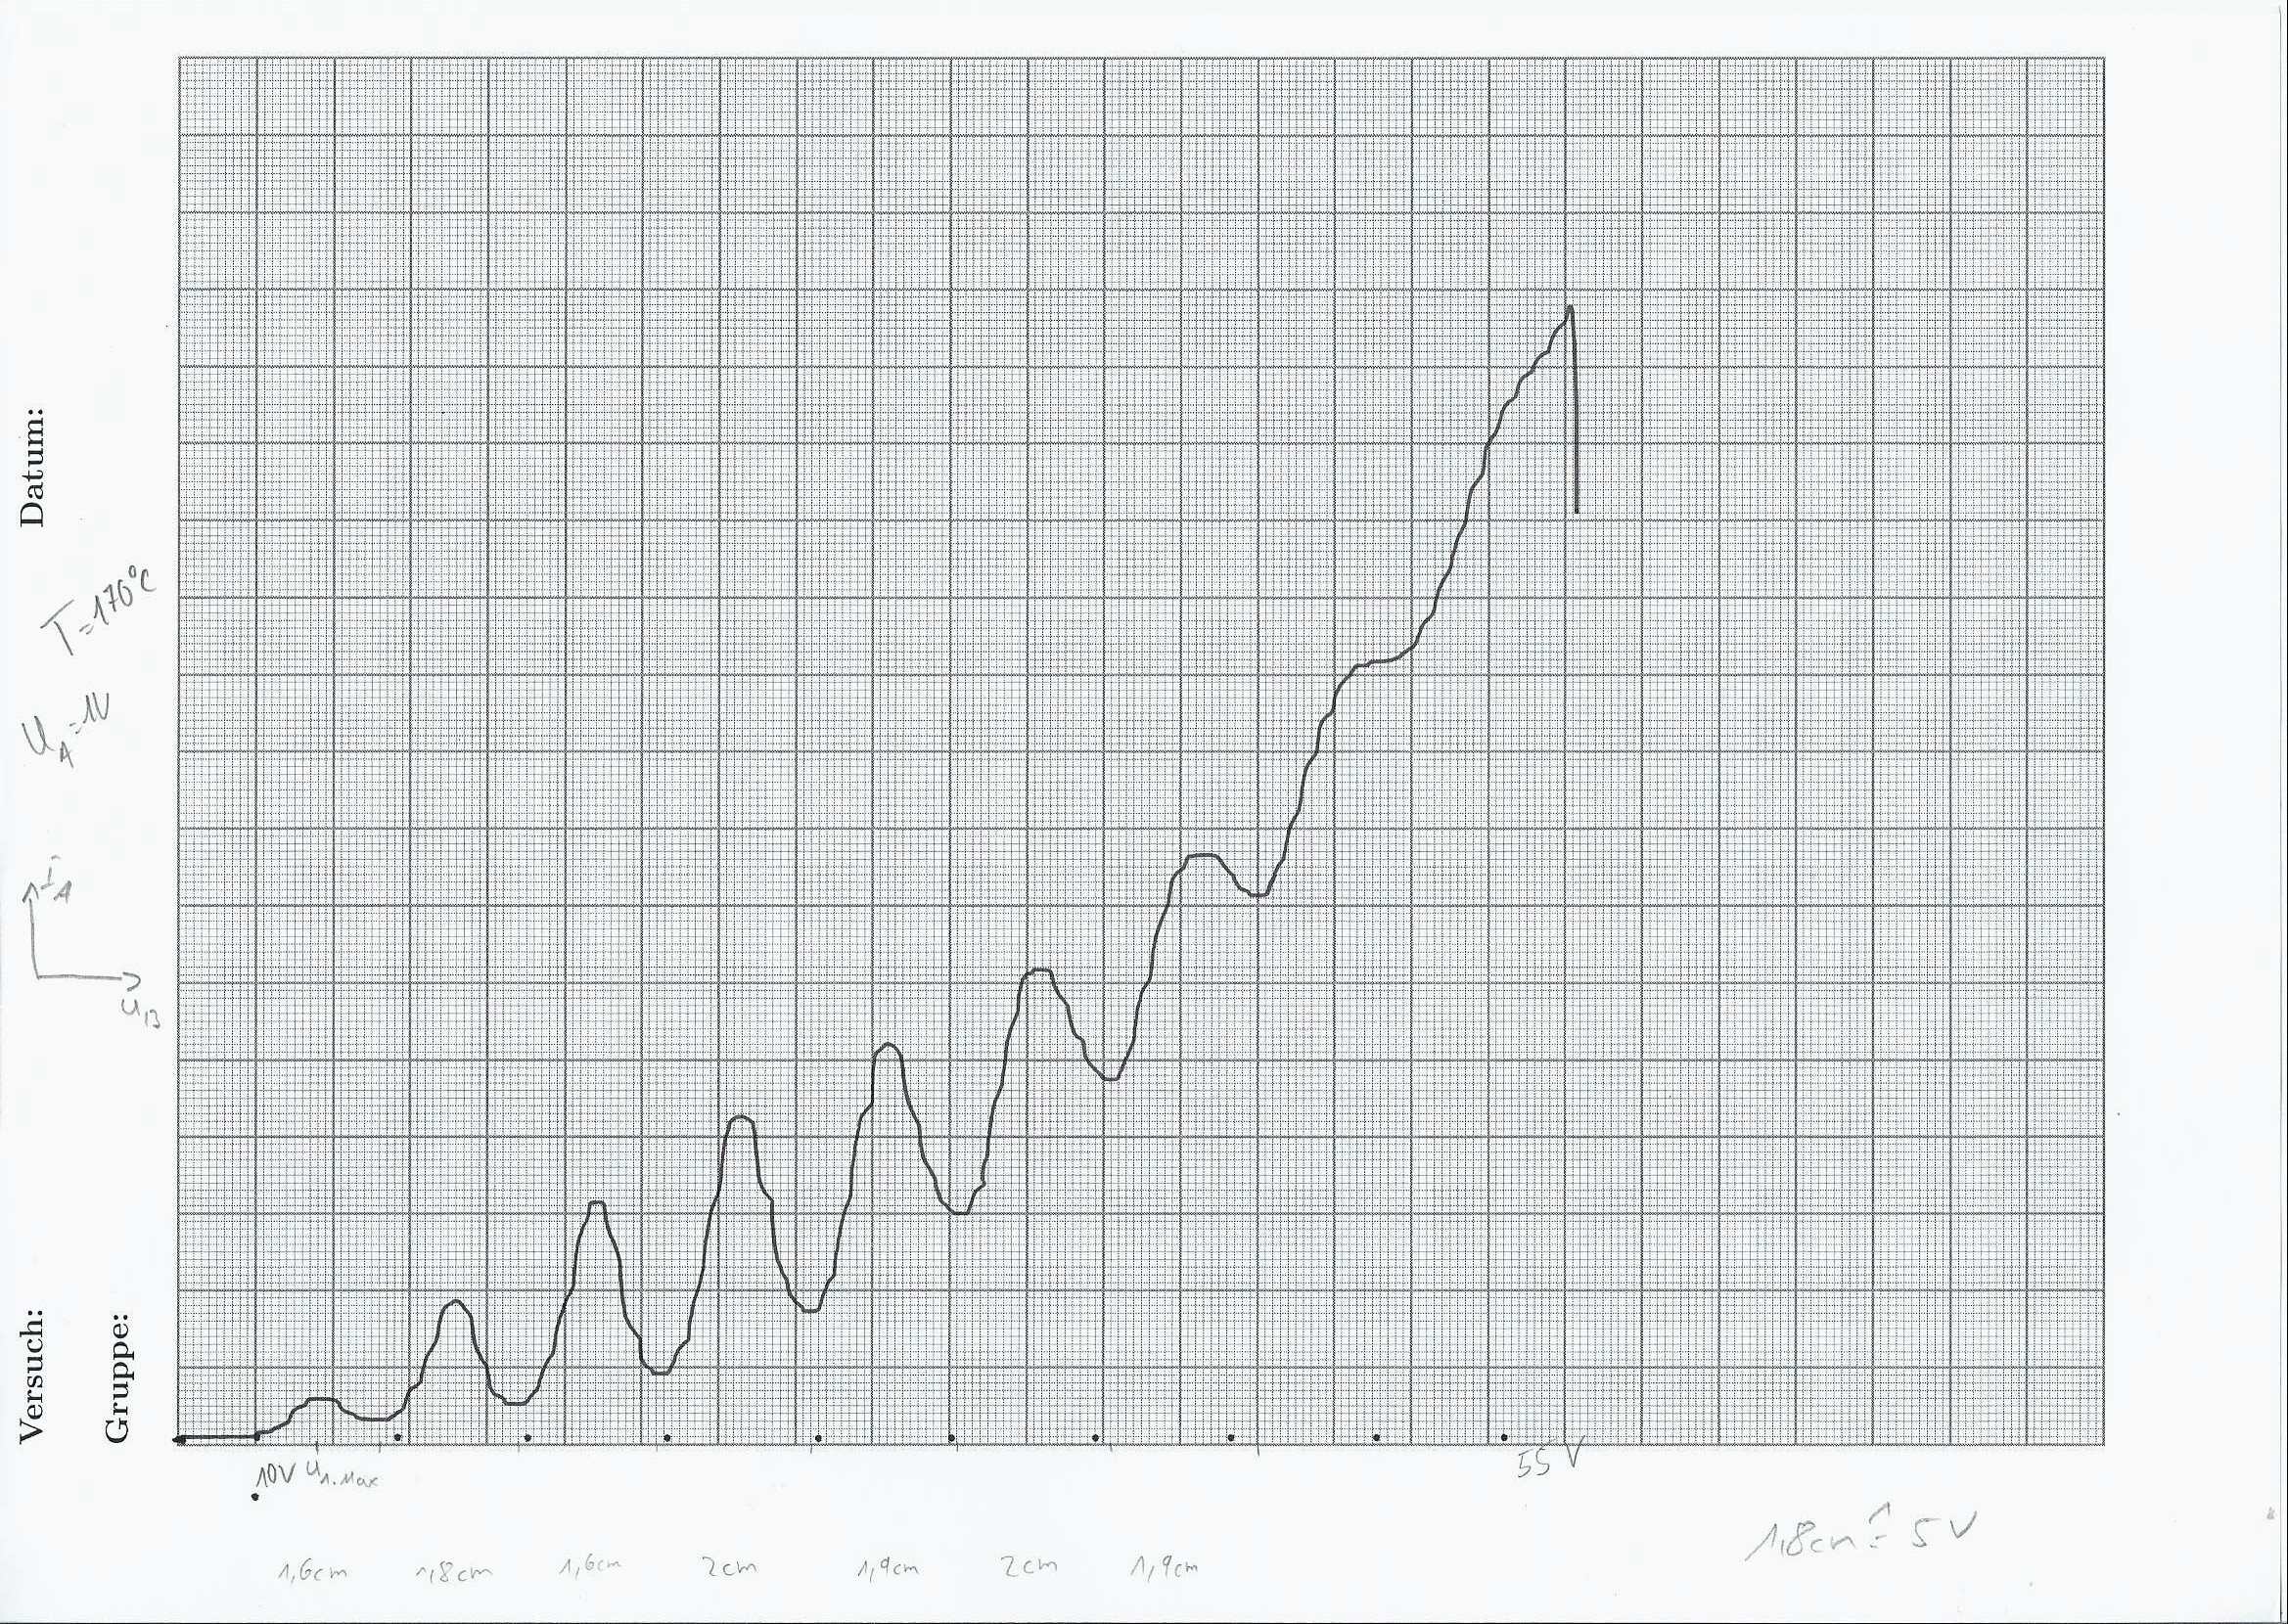
\includegraphics[width=0.8\textwidth]{bilder/kurve.pdf}
  \caption{Idealisierte Franck-Hertz-Kurve zwischen $I_A$ und $U_B$
  \cite{601}.}
  \label{fig:kurve}
\end{figure}
Der Abstand zweier Maxima $U_1$ ist gleich dem ersten Anregungspotential
\begin{equation*}
  U_1:=\frac{1}{e_0}(E_1-E_0)
\end{equation*}
des Quecksilber-Atoms.
Der tatsächliche Verlauf der Franck-Hertz-Kurve aus Abbildung \ref{fig:kurve}
wird von verschiedenen Nebeneffekten beeinflusst.

Da die Austrittsarbeit für Elektronen verschieden ist, unterscheidet sich das
tatsächliche Beschleunigungspotential von U_\su{B}.
Damit die Emissionsrate auch bei kleinen Temperaturen hoch ist, muss die
Austrittsarbeit des Drahts $\Phi_\su{G}$ viel kleiner sein als die
Austrittsarbeit der Beschleunigungselektrode $\Phi_\su{B}$.
\newpage
Abbildung \ref{fig:pot} zeigt die Potentialverhältnisse zwischen beiden Elektroden
\begin{figure}
  \centering
  \includegraphics[width=0.8\textwidth]{bilder/potential.pdf}
  \caption{Potentialverhältnisse zwischen Glühkathode und Beschleunigungselektrode
  \cite{601}.}
  \label{fig:pot}
\end{figure}
Nach dieser Abbildung berechnet sich das tatsächliche Beschleunigungspotential
mittels
\begin{equation}
  U_\su{B,eff}=U_\su{B}-\frac{1}{e_0}(\Phi_\su{B}-\Phi_\su{G}).
\end{equation}
Das Kontaktpotential
\begin{equation}
  K:= \frac{1}{e_0}(\Phi_\su{B}-\Phi_\su{G})
\end{equation}
gibt die Verschiebung der Franck-Hertz-Kurve an.

Desweiteren wurde bisher angenommen, dass die Elektronen nach durchlaufen des
Beschleunigungsraums alle die eine einheitliche Energie besitzen. Da die
Leitungselektronen bereits ein Potential besitzen, treten sie bei der
Glühemission mit unterschiedlichen Anfangsgeschwindigkeiten aus.
Die Leitungselektronen besitzen nach dem Durchlaufen des Beschleunigerpotentials $U_\su{B,eff}$
eine bei $U_\su{B} beginnende Energieverteilung, welche sich zu höheren Energien erstrecken kann.
Das führt dazu, dass sich der Ort der elastischen
Stöße über einen unendlichen Einsatzbereich erstrecken. Die Franck-Hertz-Kurve nähert sich einem
Stromminimum an und fällt nicht, wie in Abbildung \ref{fig:kurve} auf einen Ausgangswert von $0$
zurück. 
Die elastischen Stöße führen zu einer Abflachung und Verbreiterung
der Kurve, sofern sie zwischen den beiden Elektroden stattfinden.

Ein weiterer Nebeneffekt, der die Kurve beeinflusst, ist der Dampfdruck.

Damit die nötigen Zusammenstöße zwischen Elektronen und Hg-Atomen in hohem Maße
auftreten, muss die mittlere Weglänge $\bar w$ sehr klein gegen den Abstand $a$
zwischen Kathode und Beschleunigungselektrode sein. Die Weglänge kann über
den Sättigungsdruck eingestellt werden. Aus der kinetischen Gastheorie folgt der
Zusammenhang
\begin{equation}
  \bar w = \frac{0.0029}{\su{p_{sät}}}
  \label{eqn:wbar}.
\end{equation}

\begin{figure}
  \centering
  \includegraphics[height=0.8\textwidth]{bilder/dampf.pdf}
  \caption{Ideale Quecksilber-Dampfdruckkurve\cite{601}.}
  \label{fig:dampf}
\end{figure}
Die in Abbildung \ref{fig:dampf} gezeigte Dampfdruckkurve von Quecksilber
lässt sich mit
\begin{equation}
  \su{p_{sät}(T)=5.5\,\cdot10^{-7}\,\exp^{-6876/T}}
  \label{eqn:psat}
\end{equation}
berechnet.Die Temperatur bei welcher der Franck-Hertz-Effekt auftritt lässt sich
so berechnen.. Damit eine ausreichende Stoßwahrscheinlichkeit
gegeben ist, muss $\bar w$ um den Faktor 1000 bis 4000 kleiner sein als $a$
sein.
Somit gibt es einen Dampfdruckbereich bei dem eine optimale Arbeit der Apparatur gewährleistet ist.
Wird dieser unterschritten, steigt die Wahrscheinlichkeit, dass die Elektronen
keine Wechselwirkung erfahren.
Ist die Elektronenenergie bei ausreichend hoher Spannung größer als $E_1-E_0$,
können die Hg-Atome in höhere Niveaus angeregt werden.
ist der Sättigungsdruck zu groß, treten zu viele elastische Stöße auf und die Zahl
der Elektronen nimmt stark ab.

Das Hg-Atom besteht aus 80 Elektronen, die sich auf die abgeschlossenen Schalen
des Xe-Atoms mit 54 Elektronen, eine 4f-Schale mit 14 Elektronen und eine
5d-Schale mit 10 Elektronen verteilen. Diese Schalen sind ebenfalls abgeschlossen. Von Bedeutung
sind hierbei jedoch nur die 2s-Elektronen die sich in der Schale mit der
Hauptquantenzahl $n=6$ aufhalten. Die Spins dieser müssen wegen des
Pauli-Verbots im Grundzustand antiparallel stehen, da sonst alle 4
Quantenzahlen übereinstimmen würden.
Die beiden äußersten Elektronen des Hg-Atoms besitzen somit die
Quantenzahlen
\begin{align*}
  n_1 &= n_2 = 6, \\
  l_1 &= l_2 = 0, \\
  s_1 &= \frac{1}{2}, \\
  s_2 &= - \frac{1}{2}.
\end{align*}
Der Grundzustand besitzt demnach keine Feinstruktur, da die Gesamtspinquantenzahl
$S$ verschwindet. Unter Beibehaltung von $S=0$ sind Übergänge in angeregte
Zustände nur möglich, wenn die Hauptquantenzahl $n=6$ auf $n=7$ erhöht wird
und $l_1$ wegen der Auswahlregel von 0 auf 1 übergeht. Wird die Anforderung
$S=0$ vernachlässigt, lässt sich ein Niveau erzeugen, bei dem beide Spins
parallel stehen. Hierfür muss zudem der Bahndrehimpuls eines der beiden
Elektronen um 1 ändern, womit $L=1$ gilt. Das so entstandene Niveau besitzt
eine Feinstruktur aus 3 Niveaus, da 3 verschiedene Kombinationen von
$\su{\vec{L}}$ und $\su{\vec{S}}$ vorhanden sind, die zu einem Gesamtrehimpuls
$\su{\vec{J}}$ führen. Durch die Parallelstellung der Spins vermindert sich
die potentielle Energie der Elektronenhülle, da die Elektronen sich gegenseitig
"ausweichen". Das hat zur Folge, dass die Niveaus mit $n=7$ und $S=0$ unterhalb
dem Niveau mit $n=7$ und $S=1$ liegen. Die nachfolgenden Abbildung \ref{fig:termschema}
veranschaulicht die auftretenden Energierelationen.
\begin{figure}
  \centering
  \includegraphics[width=0.7\textwidth]{bilder/term.jpg}
  \caption{Theoretisches Termschema eines Hg-Atoms \cite{601}.}
  \label{fig:termschema}
\end{figure}
Der eingezeichnete Übergang vom Grundzustand in den 1. angeregten Zustand und
wieder zurück ist bei Atomen mit kleiner Ordnungszahl $z$, wie etwa Helium,
praktisch unmöglich. Bei Atomen mit großer Ordnungszahl, zum Beispiel Hg, ist
dieser Vorgang nur mit geringer Wahrscheinlichkeit zu beobachten, da er mit dem
Umklappen  eines Elektronenspins, also $\Delta s=1$, verbunden ist. Beim
Franck-Hertz-Experiment ist dies jedoch möglich, da die Anregung durch
Elektronenstoß erfolgt. Das stoßende Elektron wird hier gegen eines der beiden
6s Elektronen ausgetauscht, deren Spinrichtung entgegengesetzt ist.
